%\documentclass[10pt]{beamer} % aspect ratio 4:3, 128 mm by 96 mm
\documentclass[10pt,aspectratio=169]{beamer} % aspect ratio 16:9

%\graphicspath{{../../figures/}}
\graphicspath{{figs/}{../../figures/}{../../../reports/figures/png/}}
%\includeonlyframes{frame1,frame2,frame3,frame4,frame5,frame6,frame7,frame8,frame9}
%\includeonlyframes{frame10,frame11,frame12,frame13}
%\includeonlyframes{frame14,frame15,frame16,frame17,frame18,frame19,frame20,frame21}
%\includeonlyframes{frame22,frame23,frame24,frame25,frame26}
%\includeonlyframes{frame27,frame28}
%%%%%%%%%%%%%%%%%%%%%%%%%%%%%%%%%%%%%%%%%%%%%%%%%%
% Packages
%%%%%%%%%%%%%%%%%%%%%%%%%%%%%%%%%%%%%%%%%%%%%%%%%%
\usepackage{appendixnumberbeamer}
\usepackage{booktabs}
\usepackage{pgfplots}
\usepackage{xspace}
\usepackage{amsmath}
\usepackage{multirow}
\usepackage{totcount}
\usepackage{tikz}
\usepackage[T1]{fontenc}
\usepackage{ragged2e}

\usepackage{wrapfig}
%\usepackage{comment}
%\usetikzlibrary{external} % speedup compilation
%\tikzexternalize % activate!
%\usetikzlibrary{shapes,arrows}  

%\usepackage{bibentry}
%\nobibliography*
\usepackage{caption}%
\captionsetup[figure]{labelformat=empty}%
%%%%%%%%%%%%%%%%%%%%%%%%%%%%%%%%%%%%%%%%%%%%%%%%%%
% Metropolis theme custom modification file
%%%%%%%%%%%%%%%%%%%%%%%%%%%%%%%%%%%%%%%%%%%%%%%%%%
% Metropolis theme custom modification file
%%%%%%%%%%%%%%%%%%%%%%%%%%%%%%%%%%%%%%%%%%%%%%%%%%
% Metropolis theme custom colors
%%%%%%%%%%%%%%%%%%%%%%%%%%%%%%%%%%%%%%%%%%%%%%%%%%
\usetheme[progressbar=foot]{metropolis}
\useoutertheme{metropolis}
\useinnertheme{metropolis}
\usefonttheme{metropolis}
\setbeamercolor{background canvas}{bg=white}

%\usecolortheme{spruce}

\definecolor{myblue}{rgb}{0.19,0.55,0.91}
\definecolor{mediumblue}{rgb}{0,0,205}
\definecolor{darkblue}{rgb}{0,0,139}
\definecolor{Dodgerblue}{HTML}{1E90FF}
\definecolor{Navy}{HTML}{000080} % {rgb}{0,0,128}
\definecolor{Aliceblue}{HTML}{F0F8FF}
\definecolor{Lightskyblue}{HTML}{87CEFA}
\definecolor{logoblue}{RGB}{1,67,140}
\definecolor{Purple}{HTML}{911146}
\definecolor{Orange}{HTML}{CF4A30}

\setbeamercolor{progress bar}{bg=Lightskyblue}
\setbeamercolor{progress bar}{ fg=logoblue} 
\setbeamercolor{frametitle}{bg=logoblue}
\setbeamercolor{title separator}{fg=logoblue}
\setbeamercolor{block title}{bg=Lightskyblue!30,fg=black}
\setbeamercolor{block body}{bg=Lightskyblue!15,fg=black}
\setbeamercolor{alerted text}{fg=Purple}
%%%%%%%%%%%%%%%%%%%%%%%%%%%%%%%%%%%%%%%%%%%%%%%%%%
%  Theme modifications
%%%%%%%%%%%%%%%%%%%%%%%%%%%%%%%%%%%%%%%%%%%%%%%%%%
% modify progress bar linewidth
\makeatletter
\setlength{\metropolis@progressinheadfoot@linewidth}{2pt} 
\setlength{\metropolis@titleseparator@linewidth}{1pt}
\setlength{\metropolis@progressonsectionpage@linewidth}{1pt}

\setbeamertemplate{progress bar in section page}{
	\setlength{\metropolis@progressonsectionpage}{%
		\textwidth * \ratio{\thesection pt}{\totvalue{totalsection} pt}%
	}%
	\begin{tikzpicture}
	\fill[bg] (0,0) rectangle (\textwidth, \metropolis@progressonsectionpage@linewidth);
	\fill[fg] (0,0) rectangle (\metropolis@progressonsectionpage, \metropolis@progressonsectionpage@linewidth);
	\end{tikzpicture}%
}
\makeatother
\newcounter{totalsection}
\regtotcounter{totalsection}

\AtBeginDocument{%
	\pretocmd{\section}{\refstepcounter{totalsection}}{\typeout{Yes, prepending was successful}}{\typeout{No, prepending was not successful}}%
}%
%%%%%%%%%%%%%%%%%%%%%%%%%%%%%%%%%%%%%%%%%%%%%%%%%%
%  Bibliography mods
%%%%%%%%%%%%%%%%%%%%%%%%%%%%%%%%%%%%%%%%%%%%%%%%%%
\setbeamertemplate{bibliography item}{\insertbiblabel} %% Remove book symbol from references and add number in square brackets
% kill the abominable icon (without number)
%\setbeamertemplate{bibliography item}{}
%\makeatletter
%\renewcommand\@biblabel[1]{#1.} % number only
%\makeatother
% remove line breaks in bibliography
\setbeamertemplate{bibliography entry title}{}
\setbeamertemplate{bibliography entry location}{}
%%%%%%%%%%%%%%%%%%%%%%%%%%%%%%%%%%%%%%%%%%%%%%%%%%
%  Bibliography custom commands
%%%%%%%%%%%%%%%%%%%%%%%%%%%%%%%%%%%%%%%%%%%%%%%%%%
\newcommand{\bibliotitlestyle}[1]{\textbf{#1}\par}

\newif\ifinbiblio
\newcounter{bibkey}
\newenvironment{biblio}[2][long]{%
    %\setbeamertemplate{bibliography item}{\insertbiblabel}
    \setbeamertemplate{bibliography item}{}% without numbers
	\setbeamerfont{bibliography item}{size=\footnotesize}
	\setbeamerfont{bibliography entry author}{size=\footnotesize}
	\setbeamerfont{bibliography entry title}{size=\footnotesize}
	\setbeamerfont{bibliography entry location}{size=\footnotesize}
	\setbeamerfont{bibliography entry note}{size=\footnotesize}
	\ifx!#2!\else%
	\bibliotitlestyle{#2}%
	\fi%
	\begin{thebibliography}{}%
		\inbibliotrue%
		\setbeamertemplate{bibliography entry title}[#1]%
	}{%
		\inbibliofalse%
		\setbeamertemplate{bibliography item}{}%
	\end{thebibliography}%
}

\newcommand{\biblioref}[5][short]{
	\setbeamertemplate{bibliography entry title}[#1]
	\stepcounter{bibkey}%
	\ifinbiblio%
	\bibitem{\thebibkey}%
	#2
	\newblock #4
	\ifx!#5!\else\newblock {\em #5}, #3 \fi%
	\else%
	\begin{biblio}{}
		\bibitem{\thebibkey}
		#2
		\newblock #4
		\ifx!#5!\else\newblock {\em #5}, #3\fi
	\end{biblio}
	\fi
}
%
%\newbibmacro*{hypercite}{%
%	\renewcommand{\@makefntext}[1]{\noindent\normalfont##1}%
%	\footnotetext{%
%		\blxmkbibnote{foot}{%
%			\printtext[labelnumberwidth]{%
%				\printfield{prefixnumber}%
%				\printfield{labelnumber}}%
%			\addspace
%			\fullcite{\thefield{entrykey}}}}}
%
%\DeclareCiteCommand{\hypercite}%
%{\usebibmacro{cite:init}}
%{\usebibmacro{hypercite}}
%{}
%{\usebibmacro{cite:dump}}
%
%% Redefine the \footfullcite command to use the reference number
%\renewcommand{\footfullcite}[1]{\cite{#1}\hypercite{#1}}
%%%%%%%%%%%%%%%%%%%%%%%%%%%%%%%%%%%%%%%%%%%%%%%%%%
% Custom commands
%%%%%%%%%%%%%%%%%%%%%%%%%%%%%%%%%%%%%%%%%%%%%%%%%%
% matrix command 
\newcommand{\matr}[1]{\mathbf{#1}} % bold upright (Elsevier, Springer)
%\newcommand{\matr}[1]{#1}          % pure math version
%\newcommand{\matr}[1]{\bm{#1}}     % ISO complying version
% vector command 
\newcommand{\vect}[1]{\mathbf{#1}} % bold upright (Elsevier, Springer)
% bold symbol
\newcommand{\bs}[1]{\boldsymbol{#1}}
% derivative upright command
\DeclareRobustCommand*{\drv}{\mathop{}\!\mathrm{d}}
\newcommand{\ud}{\mathrm{d}}
% 
\newcommand{\themename}{\textbf{\textsc{metropolis}}\xspace}
%%%%%%%%%%%%%%%%%%%%%%%%%%%%%%%%%%%%%%%%%%%%%%%%%%
%  Title page options
%%%%%%%%%%%%%%%%%%%%%%%%%%%%%%%%%%%%%%%%%%%%%%%%%%
% \date{\today}
%%%%%%%%%%%%%%%%%%%%%%%%%%%%%%%%%%%%%%%%%%%%%%%%%%
% option 1
%%%%%%%%%%%%%%%%%%%%%%%%%%%%%%%%%%%%%%%%%%%%%%%%%%
\title{Odpowiedzi do pytań i uwag zawartych w recenzji z~dnia 11~czerwca~2023 dra hab. inż. Pawła Paćko, prof. AGH}
\author{\textbf{Piotr Fiborek}}
% logo align to Institute 
\institute{Institute of Fluid Flow Machinery\\Polish Academy of Sciences \\ \vspace{-1.5cm}\flushright 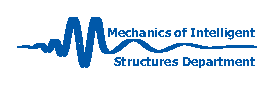
\includegraphics[width=4cm]{logo_eng_40mm.eps}}
%%%%%%%%%%%%%%%%%%%%%%%%%%%%%%%%%%%%%%%%%%%%%%%%%%
\begin{document}
	%%%%%%%%%%%%%%%%%%%%%%%%%%%%%%%%%%%%%%%%%%%%%%%%%%
	\maketitle
\begin{frame}[label=frame1]{Uwagi ogólne - Rozdział 1.}
\textit{We wprowadzeniu do pracy zabrakło, w mojej ocenie, poruszenia następujących kwestii:\\
(\textbf{a}) Analizy struktury kompozytu typu HSC jako struktury periodycznej, a zatem wykazującej charakterystyczne cechy dynamiczne. Cechy te mogą w sposób znaczący
wpływać na dobór technik badawczych i możliwość późniejszego monitorowania tego
typu struktur (poprzez np. występowanie pasm silnie tłumionych)}.\\
\textcolor{blue}{(\textbf{a}) Jest to cenny komentarz, który należałoby uwzględnić w wprowadzeniu do mojej pracy. Analiza struktury kompozytu typu HSC jako struktury periodycznej jest istotnym zagadnieniem, które może wpłynąć na wybór odpowiednich technik badawczych oraz na możliwość monitorowania takiej struktury w późniejszym okresie. Należy jednak podkreślić, że sygnały 5-cyklowe wykazują szerokie spektrum w połowie maksymalnej amplitudy, odpowiednio 20, 40 i 60 kHz dla poszczególnych sygnałów. Analiza Rysunku \ref{fig:signal_spectrum} pozwala zauważyć, że w badanej strukturze brakuje wystarczająco szerokich pasm tłumionych, które mogłyby całkowicie wytłumić rozchodzącą się falę.}
\end{frame}

\begin{frame}
	\begin{figure}
		\centering
		\caption{Spektrum sygnały szerokopasmowego zarejestrowany przez czujnik wraz z charakterystyką trzech sygnałów 5-cyklowych}
		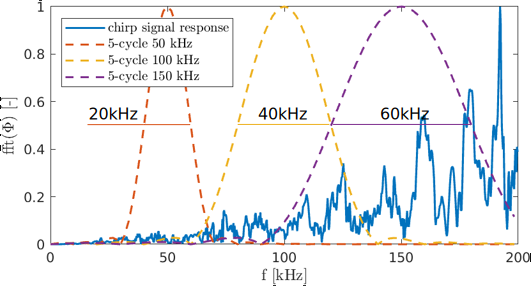
\includegraphics[width=0.8\textwidth]{figs/sensor_response_frequency_domain}
		\label{fig:signal_spectrum}
	\end{figure}
\end{frame}
\begin{frame}[label=frame2]{Uwagi ogólne - Rozdział 1.}\justifying
\textit{(\textbf{b}) Analizy charakterystyki panelu HSC pod kątem specyfiki fal prowadzonych w nim propagujących, szczególnie w kontekście rodzajów postaci fal (A0 /S0 i inne). Czy postacie o takiej symetrii będą propagować w asymetrycznej strukturze? Jak wyglądają charakterystyki wzbudzalności i tłumienia (o ile zakłada się tłumienie w materiałach będących składowymi kompozytu)? Silne tłumienie fal krótkich w tego typu strukturach może znacznie utrudniać ich monitorowanie.}\\
\textcolor{blue}{(\textbf{a}) Mody A0 i S0 to fundamentalne postacie fal Lamba o asymetrycznym i symetrycznym rozkładzie przemieszczeń w przekroju poprzecznym elementu, w którym się propagują. Naturalnie, taki idealny rozkład przemieszczeń może wystąpić jedynie w konstrukcjach o symetrycznych własnościach materiałowych i warunkach brzegowych. Mody propagujące w analizowanej konstrukcjach wykazują podobieństwo do teoretycznych modów A0 i S0 fal Lamba. Przykładowo, wyższa prędkość grupowa modu S0, przemieszczenia dla niskich częstotliwościach dominuje w kierunku poprzecznym dla modu A0 i wzdłużnym dla modu S0, większa dyspersja modu A0.}
\end{frame}

\begin{frame}[label=frame3]{Uwagi ogólne - Rozdział 1.}\justifying
\textcolor{blue}{W dysertacji, wartość współczynnika proporcjonalności macierzy tłumienia została ustalona poprzez dostrojenie odpowiedzi modelu referencyjnego w temperaturze pokojowej do pomiarów eksperymentalnych. Wartości tłumienia zostały dostosowane indywidualnie tylko dla płyty CFRP w zależności od każdej z częstotliwości wymuszenia. Wartości współczynnika były różne dla przemieszczeń w kierunku osi X i Y, które w~głównej mierze odpowiadają za tłumienie modu S0, oraz dla kierunku osi Z, który jest związany z tłumieniem modu A0. Dla symulacji próbek z uszkodzeniami oraz analizy wpływu temperatury otoczenia przyjęto wartości referencyjne, które przedstawione są w Tabeli \ref{tab:damp}.
\begin{table}[!hbt]
	\tabcolsep=0.1cm
	\centering
	\caption{\label{tab:damp} Wpspółczynniki tłumienia dla płyty CFRP}
	\begin{tabular}{cccc}
		\textbf{Frequency} & \multicolumn{3}{c}{\(\alpha_M\times 10^3\)} \\
		\([\mathrm{kHz}]\) & x & y & z\\\midrule
		50 & 1 & 1 & 5\\
		100 & 10 & 10 & 24\\
		150 & 50 & 50 & 500
	\end{tabular}
\end{table}
}
\end{frame}
\begin{frame}
	\begin{figure}
		\centering
		\caption{Krzywe wzbudzalności modów A0 i S0.}
		\includegraphics[width=0.8\textwidth]{figs/excitability}
		\label{fig:excitability}
	\end{figure}
\end{frame}
\begin{frame}[label=frame4]{Uwagi ogólne - Rozdział 2.}\justifying
\textit{W rozdziale drugim Autor dokonał syntezy głównych wątków poruszonych w rozdziale
pierwszym i na tej podstawie sformułował problem badawczy. Nie mam uwag ogólnych do tego rozdziału.}
\end{frame}
\begin{frame}[label=frame5]{Uwagi ogólne - Rozdział 3.}\justifying
\textit{W rozdziale trzecim brakuje nieco przejrzystości:\\
(\textbf{a}) Nie jest na przykład jasne, które modele podlegają dostrojeniu – najbardziej zasadnym byłoby przyjąć, że są to modele bez uszkodzenia, które są dostrajane do wyników eksperymentu fizycznego, a następnie wprowadzane są do nich uszkodzenia (wmodelu). Wniosek przeciwny sugerowałby, że model nie dostarcza nowej wiedzy na temat interakcji fal z uszkodzeniem, a jest jedynie dostrajany, aby uzyskać wyniki zgodne z eksperymentem fizycznym.}
\end{frame}
\begin{frame}[label=frame6]{Uwagi ogólne - Rozdział 3.}\justifying
\textcolor{blue}{(\textbf{a}) Zgadzam się, że konieczne jest bardziej klarowne określenie, które modele podlegają dostrojeniu. W dysertacji, tylko model referencyjny bez uszkodzenia w temperaturze \(+20^{\circ}C\) zostal dostrajony do wyników eksperymentu fizycznego. Następnie symulacje dla próbek z uszkodzeniem realizowane są z parametrami ustalonymi dla próbki referencyjnej. Wynika to bezpośrednio z Rys. 3.6, ale w celu uniknięcia wszelkich wątpliwości i niejasności, w sekcji 3.3 (linia 4) zdanie} "\textit{If the simulation results did not agree with the measured results, the material parameters of the components were adjusted.}", \textcolor{blue}{powinno być zastopione przez: "If the simulation results did not agree with the measured results, the material parameters of the reference model (pristine sample at \(+20^{\circ}C\)) components were adjusted.}"
\end{frame}
\begin{frame}[label=frame7]{Uwagi ogólne - Rozdział 4.}\justifying
\textit{Rozdział czwarty wprowadza czytelnika w podstawy „metody elementów spektralnych”, wspomagając zrozumienie dalszych części pracy i opisywanych tam badań i ich wyników. Nasuwają się w związku z tym następujące pytania:\\
(\textbf{a}) W rozdziale czwartym Autor opisuje de facto metodę elementów skończonych, w której 	wykorzystywane są wielomiany Legendre’a i w specyficzny sposób dobierane jest położenie węzłów elementu. W efekcie uzyskuje się skupioną macierz mas, która – podobnie do klasycznego podejścia – umożliwia rozprzęgnięcie układu równań i ich przetwarzanie równoległe, co przekłada się na możliwość znacznej redukcji czasu obliczeń. W literaturze funkcjonują jednak dwie metody „spektralne”, które czasami mogą być mylone. Z tego też powodu przyjęło się (choć zasada ta nie zawsze jest przestrzegana), że metodę opisywaną przez Doktoranta określa się jako spektralną metodę elementów skończonych, z ang. SFEM, w odróżnieniu do metody elementów spektralnych, z ang. SEM, w której funkcje kształtu są jawnie zależne od częstotliwości.}
\end{frame}
\begin{frame}[label=frame8]{Uwagi ogólne - Rozdział 4.}\justifying
\textcolor{blue}{(\textbf{a}) W dysertacji zastosowałem termin "spektralna metoda elementów skończonych (SEM)", która została użyta w pionierskiej pracy A. Patera dotyczącej obliczeń przepływów laminarnych [Patera, 1984]. Metoda SEM jest połączeniem klasycznej metody elementów skończonych oraz metod z funkcjami kształu zależnymi od częstotliwości. Jednakże zgadzam się, że obecnie często spotyka się w literaturze światowej oznaczenie zastosowanej metody jako SFEM, dla rozróżnienia obu metod.}\\
\textit{(\textbf{b}) Autor opisuje swoją metodę łączenia elementów skończonych typu 3-D i 2-D, jednak nie odnosi się do podobnych problemów i sposobów ich rozwiązania w znanych metodach takich jak np. MES. Czym różnią się metody łączenia tego typu elementów stosowane w MES (np. w rozwiązaniach komercyjnych) i czy mogłyby być wprost zaimplementowane w SFEM? Jakie mogłyby być różnice wynikające ze specyficznej formulacji SFEM?}
\end{frame}

\begin{frame}[label=frame9]{Uwagi ogólne - Rozdział 4.}\justifying
\textcolor{blue}{(\textbf{b}) Zaimplementowana metoda połączenia elementów bazuje na metodach stosowanych w FEM z zastosowanie mnożników Lagrange'a [Farhat i Roux, 1991]. Ashwin i inni [Ashwin, 2014] zaimplenentował interfejst pomiędzy elementami płytowymi dla elementów o zgodnych węzłach. W mojej pracy zaimplementowałem interfejs dla niepasujących siatek. Idea jest podobna do rozwiązań stosowanych w FEM, a zasadnicza różnica jest w wyborze funkcji interpolacyjnej. Przykładowo w FEM stosowane są liniowa funkcja kształtu, funkcja wielomianu stopnia trzeciego lub funkcja stała [Flemisch, 2006]. W przypadku komercyjnego programu Abaqus, nie odnalazłem w dokumentacji użytkownika stosownego komentarza w kwestii zastosowanej funkcji.\\}
\textit{(\textbf{c}) W rozdziale 4.9 Autor odnosi się do macierzy o dużych rozmiarach oraz problemów związanych z wykonywaniem na nich operacji. Dla problemów liniowych, takich jak w analizowanym w pracy przypadku, efektywne są metody, w których macierzy w ogóle się nie agreguje, ale rozwiązuje problem na poziomie elementów (równolegle), a dopiero odpowiedź modelu rekonstruuje się z tych składowych. Czy tego rodzaju metody były rozważane do rozwiązania problemów analizowanych w ramach rozprawy? Jakie mogłyby być ich zalety i wady w stosunku do tych wykorzystanych w pracy?\\}
\end{frame}
\begin{frame}[label=frame10]{Uwagi ogólne - Rozdział 4.}\justifying
\textcolor{blue}{(\textbf{c})  W rozprawie zastosowano rozwiązanie na poziomie elementów, które zostało zaimplementowanow SFEM w [Kudela, 2016]. Zamiast zagregowanej macierzy sztywności zapisuje się w postaci macierzy równania dla każdego elementu niezależnie. Dzięki temu obliczenie sił wewnetrznych realizowane jest poprzez mnożenie odpowiadającym sobie elementów odpowiednio zaimplementowanych macierzy, unikając czasochłonnej operacji mnożenia macierzowego macierzy sztywności przez wektor przemieszczeń. W sekcji 4.9 zaprezentowałem udoskonalenie algorytmu zaprezentowanego w [Kudela, 2016], aby jeszcze bardziej przyspieszyć całkowanie równania ruchu po czasie.}\\
\textit{(\textbf{d}) W sekcji 4.11 Autor stwierdza, że bez zaproponowanego przez niego elementu pośredniego połączenie elementów 3-D i 2-D byłoby bardzo trudne. Czy możliwe byłoby wykorzystanie klasycznych metod redukcji obciążeń pozawęzłowych do węzłowych i wykorzystanie mnożników Lagrange’a do uzyskania podobnych wyników jednak bez elementów pośrednich? Jakie mogłyby być zalety i wady takiego rozwiązania?}
\end{frame}

\begin{frame}[label=frame11]{Uwagi ogólne - Rozdział 4.}\justifying
\textcolor{blue}{(\textbf{d}) Zgadza się, sformułowanie "bardzo trudne" może być niefortunne. Moją intencją było podkreślenie, że w przypadku obecnie dostępnych implementacji metody SFEM istnieje wyzwanie związane z zachowaniem zbieżnych węzłów przy połączeniu przylegających elementów. To z kolei mogłoby prowadzić do potrzeby wygenerowania bardzo zagęszczonej siatki, co nie zawsze jest efektywne ani praktyczne. W moim rozwiązaniu interfejs oparty jest na mnożnikach Lagrange’a, który dobrze jest znany w klasycznej metodzie FEM, ale różnica polega na wykorzystaniu elementarnych funkcji kształtu. To podejście pozwala na dyskretyzację obszarów poszczególnych elementów niezależnie. Wadą tego rozwiazania jest potrzeba wykonania jednej operacji odwrócenia macierzy, co w przypadku  gęstej macierzy sprzeżenia z równania (4.35) \(\textbf{G}\mathrm{\textbf{d}}=0\) jest czasochłonne.}
\end{frame}

\begin{frame}[label=frame12]{Uwagi ogólne - Rozdział 5.}\justifying
\textit{W rozdziale piątym opisano parametry modelu numerycznego, w tym założenia dotyczące jego wielkości, przyjętych elementów oraz sygnału wymuszającego. W tej części pracy zawarto również założenia i wyniki analiz zbieżności przestrzennej i czasowej dla modelu. Rozdział jest przejrzysty i technicznie dobrze napisany. Nasuwające się uwagi i komentarze są następujące:\\
(\textbf{a}) Autor w rozdziale 5.1 przedstawia założenia dotyczące sygnału wymuszającego,
przyjmując, że będzie to sygnał sinusoidalny złożony z pięciu okresów oraz że do jego wyprofilowania amplitudowego zastosowane zostanie okno Hanna. Przyjęto trzy częstotliwości wymuszenia 50, 100 i 150 kHz. Jest to dość powszechny wybór dla cienkich struktur kompozytowych i metalowych. Zastanawia, że wybór ten nie został poprzedzony analizą charakterystyk spektralnych badanego panelu kompozytowego (krzywych dyspersji i krzywych wzbudzalności), które umożliwiłyby odpowiedni dobór długości fali oraz jej postaci do analizowanych uszkodzeń. Powstaje pytanie jakie postacie wzbudzają się i jakie są dominujące dla wybranych częstotliwości wymuszenia oraz jakie mają długości?}
\end{frame}

\begin{frame}[label=frame13]{Uwagi ogólne - Rozdział 5.}\justifying
	\begin{columns}
	\column{0.6\textwidth}
	\begin{figure}
		\centering
		\caption{Krzywe dyspersji panelu przekładkowego wyznaczone za pomocą symulacji SFEM.}
		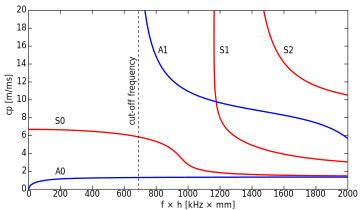
\includegraphics[width=0.9\textwidth]{figs/dispersion}
		\label{fig:dispersion}
	\end{figure}
	\column{0.4\textwidth}
	\begin{tabular}{ccc}
		\textbf{Frequency} & {\(\lambda_{A0}\)} & {\(\lambda_{S0}\)}\\
		\([\mathrm{kHz}]\) & \multicolumn{2}{c}{[mm]} \\\midrule
		50 & 20 & 98 \\
		100 & 11 & 57 \\
		150 & 8 & 36 
	\end{tabular}
\end{columns}
\end{frame}
\begin{frame}[label=frame14]{Uwagi ogólne - Rozdział 5.}\justifying
\textit{(\textbf{b}) W dalszej części rozdziału przedstawiono konfigurację badanego panelu wraz ze szczegółami jego geometrii. Na uwagę – w kontekście powyższych i dalszych uwag – zasługuje kształt rdzenia, który ma kształt heksagonalny. Periodyczność rdzenia – rzędu kilkunastu milimetrów (h1 = 11 mm) – niesie za sobą pewne konsekwencje w kontekście zjawisk falowych. Jednym z efektów, które może on wywołać jest powstawanie pasm zabronionych dla postaci fal, których długość jest podobnego rzędu. Tym bardziej zasadna byłaby analiza charakterystyk spektralnych, która umożliwiłaby ocenę czy tego rodzaju zjawiska mogą zachodzić w badanym elemencie.}\\
\textcolor{blue}{(\textbf{b}) Na Rysunku \ref{fig:signal_spectrum} wykazano, że pasma zabronione są zbyt wąskie, aby całkowicie ograniczyć propagację wymuszonych sygnałów. Odpowiedni komentarz powinien znaleźć się w pracy.}
\end{frame}
\begin{frame}[label=frame15]{Uwagi ogólne - Rozdział 5.}\justifying
\textit{(\textbf{c}) Nieco dalej, w tym samym rozdziale, Autor pisze o równoważnym modelu jednorodnym (anizotropowym). Ciekawą byłaby dyskusja o homogenizacji modelu na podstawie reguł innych niż uśrednianie stałych sprężystości, a w analizowanym przypadku oparta o uśrednianie w kontekście ekwiwalentnych własności spektralnych. Należy zwrócić uwagę, że zaproponowany równoważny model jednorodny nie ma możliwości odwzorowania pasm zabronionych ze względu na brak periodyczności w jego strukturze. Zaproponowane metody homogenizacji są dobre dla zagadnień statycznych jednak mogą prowadzić do błędów w przypadku zjawisk falowych.}\\
\textcolor{blue}{(\textbf{c}) Zgadza się, że proponowany równoważny model jednorodny może nie odzwierciedlać pasm zabronionych ze względu na brak periodyczności w jego strukturze. To ważna uwaga i stanowi ograniczenie proponowanego modelu. W moim badaniu wybrałem uśrednianie stałych sprężystości jako metodę homogenizacji, ponieważ jest ona najczęściej spotykana metoda w analizie propagacji fal sprężystych w kompozytach przekładkowych [Grede et al. 2006, Hosseini i Gabbert 2013, Sikdar et. al 2015].  Jednak rozumiem, że istnieją także inne metody homogenizacji, takie jak uśrednianie w kontekście ekwiwalentnych własności spektralnych, które mogą być bardziej odpowiednie.}
\end{frame}
\begin{frame}[label=frame16]{Uwagi ogólne - Rozdział 5.}\justifying
\textit{(\textbf{d}) W rozdziale 5.5 opisano sposób modelowania uszkodzenia jednocześnie wskazując, że podczas jego fizycznej implementacji doszło do deformacji rdzenia. Jaki jest wpływ rozwarstwienia pomiędzy warstwą wierzchnią i rdzeniem, a jaki deformacji rdzenia na propagację fali? Czy da się wykryć i rozróżnić uszkodzenia tego rodzaju?}\\
\textcolor{blue}{(\textbf{d}) Deformacja rdzenia jest powszechnym typem uszkodzenia w kompozytach przekładkowych, często wynikającym z działania sił uderzeniowych. Przykładowo, materiały wykorzystywane w poszyciu samolotów mogą ulec zniszczeniu na skutek uderzenia gradu, kolizji z ptakiem lub wyładowań atmosferycznych. Lokalna deformacja zmienia sztywność struktury, co otwiera drogę do zastosowania metod analizy fal sprężystych w celu wykrycia takiego uszkodzenia.\\
W ramach niniejszej dysertacji przeprowadzono analizę MADIF dla dwóch różnych modeli uszkodzenia: (i) usunięcie jedynie elementów interfejsu oraz (ii) usunięcie komórek z obszaru uszkodzenia. Pierwszy model odpowiada braku deformacji rdzenia samo rozklejenie, natomiast drugi model symuluje 100\% deformację rdzenia. Na Rysunku poniżej widać wyraźne różnice w wartościach MADIF dla tych dwóch modeli uszkodzenia. Przeprowadzone symulacje dają nadzieję na możliwość rozróżnienia obu rodzajów uszkodzeń w rzeczywistych warunkach.}
\end{frame}
\begin{frame}
\begin{figure}
	\centering
	\includegraphics[width=0.8\textwidth]{figs/2damagemodel}
	\label{fig:2damagemodel}
\end{figure}
\end{frame}

\begin{frame}[label=frame17]{Uwagi ogólne - Rozdział 5.}\justifying
\textit{(\textbf{e}) W rozdziale zaprezentowano analizę zbieżności – zarówno w odniesieniu do przestrzeni jak i czasu. Jako referencję dla analizy zbieżności w kontekście stopnia wielomianu interpolacyjnego Autor przyjął 11 stopień i do tego wyniku odnosił rezultaty uzyskane w dalszej części pracy. Na jakiej podstawie uznano, że ten stopień jest wystarczająco dokładny, aby był traktowany jako punkt odniesienia? Czy analizowane były wyższe stopnie wielomianów i/lub siatki elementów skończonych o znacznie mniejszych wymiarach?}\\
\textcolor{blue}{(\textbf{e}) Wybór stopnia 11 wynikał z praktycznych ograniczeń zasobów obliczeniowych. Analiza wyższych stopni wielomianów lub elementów siatki o mniejszych wymiarach wymagałaby znacznie większych zasobów pamięciowych, które nie były dostępne na dostępnej stacji roboczej. Warto zauważyć, że na Rysunku \ref{fig:dx_conv_2} widać, że już dla wielomianów stopnia 7 wskaźnik zbieżnośći jest mniejszy niż 10\%.}
\end{frame}
\begin{frame}
\begin{figure}
	\centering
	\includegraphics[width=0.8\textwidth]{figs/dx_conv_2}
	\label{fig:dx_conv_2}
\end{figure}
\end{frame}
\begin{frame}[label=frame18]{Uwagi ogólne - Rozdział 5.}\justifying
\textit{(\textbf{f}) W tabeli 5.2 zestawiono wielkości elementów skończonych wykorzystanych dla poszczególnych komponentów modelu. Ciekawym byłoby również przytoczenie liczby stopni swobody modelu i odniesienie tych danych do modelu/rozwiązania uzyskanego za pomocą klasycznej formulacji elementów skończonych. Warto zauważyć, że na Rysunku \ref{fig:dx_conv_2} widać, że już dla wielomianów stopnia 7 wskaźnik zbieżnośći jest mniejszy niż 10\%. }\\
\textcolor{blue}{(\textbf{f}) Zestawienie liczby stopni swobody modelu i jego porównania z klasyczną formulacją elementów skończonych mogłoby dostarczyć cennych informacji na temat dokładności i efektywności proponowanego modelu. Jednak, postanowiłem nie zawierać takiego porównania ponieważ, aby tego dokonać za pomocą opracowanego przeze mnie algorytmu do analizy SFEM, musiałbym zmienić proces dyskretyzacji struktur symulacji oraz niewielkie zmiany w wyborze węzłów całkowania. Ponadto, w literaturze dokonano wiele porównań obu metod, wykazując znacznie szybszą zbieżność SEM. Przykładem jest pracy [Willberg et al. 2012].}
\end{frame}
\begin{frame}[label=frame19]{Uwagi ogólne - Rozdział 5.}\justifying
\textit{(\textbf{g}) Analiza przedstawiona na stronie 47, odnosząca się do rysunku 5.6 wymaga dyskusji. Jako kryterium zbieżności przyjęto wskaźnik dany równaniem (5.2), który bazuje na obwiedni sygnału czasowego. Wskaźnik ten jest zatem zależny od długości okna i różnicy w sygnałach czasowych pomiędzy symulacjami. Wskaźniki oparte o bezpośrednie porównanie sygnałów czasowych mają wiele wad, jak na przykład dużą wrażliwość na przesunięcia fazowe. Czy zatem z praktycznego punktu widzenia można (czy warto?) rozważyć inne wskaźniki do oceny zbieżności? Dużą różnicę w sygnałach czasowych, a co za tym idzie we wskaźniku (5.2) zauważyć można dla chwil czasowych w pobliżu 200 us. Czy różnica ta mogła wynikać z nakładania się (konstruktywnego) fal odbitych od krawędzi modelu? Wynik ten zdaje się odstawać od innych w sposób znaczący, co potwierdza rys. 5.6b. Jakie może być wyjaśnienie tego specyficznego zjawiska (niemonotonicznego w funkcji stopnia wielomianu interpolującego).}
\end{frame}
\begin{frame}[label=frame19]{Uwagi ogólne - Rozdział 5.}\justifying
\textcolor{blue}{(\textbf{g}) \small{Przede wszystkim warto rozważyć wydłużenie całkowitego okresu propagowania fali do 1600 \(\mu\)s, tak jak w przypadku analizy MADIF, w celu większego wytłumienia modów. Na rysunku poniżej przedstawiłem porównanie zbieżności rozwiązania z dysertacji dla dłuższego czasu. Dodatkowo, warto rozważyć wyznaczenie indeksów RMSD i CC, które zostały zastosowane do wyznaczenia wskaźnika MADIF. Te indeksy mogą dostarczyć dodatkowych informacji na temat zbieżności symulacji. Należy zauważyć, że znaczne różnice amplitudy sygnałów w okolicy 200 \(\mu\)s mogą mieć wpływ na niemonotoniczność otrzymanej funkcji. W przypadku wartości parametru p=5 można zauważyć zbyt duże wartości, podczas gdy dla p=4 wartości są zbyt małe w porównaniu do pozostałych stopni wielomianu. Te różnice mogą również wynikać ze specyficznej interferencji fal odbitych od brzegu panelu.}}
\end{frame}
\begin{figure}
	\centering
	\includegraphics[width=0.6\textwidth]{figs/dx_conv_1600us_pp}
\end{figure}
\begin{frame}[label=frame20]{Uwagi ogólne - Rozdział 5.}\justifying
\textit{(\textbf{h}) Część poświęcona zbieżności czasowej, a raczej analizie stabilności układu jest dość oczywista i związana z podstawową własnością schematów jawnego całkowania po	czasie. Znalazłem tutaj dwie sprawy wymagające komentarza. Autor wskazuje, że krytyczna wielkość kroku czasowego zależy od wielkości siatki (wielkości elementu) oraz postaci fali. To dość kontrowersyjne, ponieważ model powinien być stabilny dla każdej postaci fali. Ponadto nie można zagwarantować, szczególnie w analizie przejściowej, że energia będzie ograniczona do wybranego pasma częstotliwości. Druga sprawa to przyjęty warunek stabilności. W formie przytoczonej przez Doktoranta jest to przybliżenie jednowymiarowe, dobre jako punkt startowy dla dalszej analizy. Istnieją jednak lepsze dwu- i trój-wymiarowe formuły, których wykorzystanie mogłoby zaoszczędzić Autorowi manualnego poszukiwania optymalnego kroku czasowego dla przeprowadzonych analiz numerycznych.}
\end{frame}
\begin{frame}[label=frame21]{Uwagi ogólne - Rozdział 5.}\justifying
	\begin{wrapfigure}{r}{0.45\textwidth}
		\centering
		\includegraphics[width=0.5\textwidth]{figs/dt_50kHz_400us}
		\label{fig:conv_t}
	\end{wrapfigure}
\textcolor{blue}{(\textbf{h}) W tej części pracy mogłem wyrazić się bardziej precyzyjnie. W rzeczywistości, wielkość kroku czasowego zależy zarówno od odległości między węzłami, jak i od maksymalnej prędkości składowej harmonicznej propagującej fali. Jednak w kontekście analizowanych sygnałów, takich jak sygnał sinusoidalny okienkowany funkcją Hanna, to głównie wielkość użytej siatki ma kluczowe znaczenie.
W~mojej pracy nie korzystam z metod optymalizacyjnych do wyboru kroku czasowego, ponieważ osiągam zbieżność czasową poprzez przeprowadzenie zaledwie kilku wielu symulacji, z różnymi wartościami próbkowania sygnałów o tej samej długości. Zazwyczaj wybieram ilość kroków będącą kolejnymi potęgami liczby 2, co jest stosunkowo efektywnym podejściem w praktyce. Warto również zauważyć, że na dołączonym rysunku można zaobserwować, że po przekroczeniu wartości krytycznej, wraz ze spadkiem wartości kroku czasowego, sygnał pozostaje niezmienny.}
\end{frame}
\begin{frame}[label=frame22]{Uwagi ogólne - Rozdział 6.}\justifying
\small{\textit{Uwagi natury ogólnej do rozdziału szóstego:\\
(\textbf{a}) Rozdział 6.1 wymaga wyjaśnienia. Nie jest do końca jasne jakie modele i w jakich konfiguracjach zostały ze sobą zestawione. Autor dokonał analizy charakterystyki częstotliwościowej (impedancyjnej) badanego przetwornika i porównał ją z modelem analitycznym dostępnym w literaturze (równanie (6.2)). Do porównania wykorzystano zapewne dane producenta przetwornika lub – co bardziej prawdopodobne sądząc po zgodności wyników – dopasowano charakterystykę analityczną do eksperymentalnej. Jest to praktyka zgodna z metodologią powszechnie stosowaną w analizie tego rodzaju układów. Warto podkreślić, że zarówno model analityczny jak i procedura analizatora zakłada wykorzystanie sygnału o zmiennej częstotliwości w celu uzyskania charakterystyki wyjściowej (przy czym zwykle stosuje się dość złożony sposób generowania i filtrowania sygnałów, rzadziej wykorzystywany jest wprost sygnał typu „chirp”). W tym kontekście zastanawia, dlaczego w analizie numerycznej przetwornika z wykorzystaniem SFEM zastosowano sygnał zbliżony do szerokopasmowego, o znacznie innej charakterystyce amplitudowej i wykonano analizę przejściową zamiast	harmonicznej? W implementacji SFEM zrealizowanej przez autora łatwo byłoby taką procedurę napisać, gdy zagregowane są już macierze K i M. Nieco zastanawiające są rozbieżności pomiędzy uzyskanymi numerycznie charakterystykami częstotliwościowymi, szczególnie gdy istnieje możliwość ich dopasowania w modelu	numerycznym do uzyskanej charakterystyki eksperymentalnej.}}
\end{frame}

\begin{frame}[label=frame23]{Uwagi ogólne - Rozdział 5.}\justifying
	\begin{wrapfigure}{r}{0.45\textwidth}
		\centering
		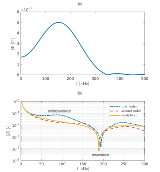
\includegraphics[width=0.5\textwidth]{figs/impedance}
		\label{fig:impedance}
	\end{wrapfigure}
\textcolor{blue}{(\textbf{a}) W analizie analitycznej oraz w symulacji komputerowej impedancji przetwornika przyjąłem wartości znamionowe dostarczone przez producenta i nie były one modyfikowane ani dostosowywane do charakterystyki eksperymentalnej. Zgadzam się, że zarówno analiza analityczna, jak i eksperymentalna analiza impedancji wykorzystują sygnały sinusoidalne o konkretnej częstotliwości. W mojej pracy, zdecydowałem się na inne podejście, korzystając z szerokopasmowego sygnału, podobnie jak w książce [Kaltenbachera, 2018], który wykorzystał sygnał trójkątny. Na rysunku obok przedstawiłem dodatkowe wyniki, uzyskane dla 20-cyklicznych sygnałów sinusoidalnych, okienkowanych funkcją Hanna. Wyniki te dokładniej oddają charakterystykę rzeczywistą. Jednakże, jedną z zalet metody zastosowanej w mojej pracy jest możliwość wyznaczenia charakterystyki za pomocą jednej symulacji, co jest praktycznym podejściem w kontekście analizy przetwornika.}
\end{frame}

\begin{frame}[label=frame24]{Uwagi ogólne - Rozdział 6.}\justifying
\textit{(\textbf{b}) Opisane w sekcji 6.2 urządzenia firmy Polytec są znane z braku mechanizmu korekcji	amplitudy mierzonej fali w związku ze zmianą kąta padania wiązki lasera na badaną powierzchnię. Czy efekt ten został uwzględniony w analizie sygnałów? Czy mógł on mieć wpływ na powstanie rozbieżności pomiędzy punktami pomiarowymi, które są od siebie znacznie oddalone?}\\
\textcolor{blue}{(\textbf{a}) Kąt padania wiązki lasera zależy od wielkości badanej próbki oraz odległości głowicy urządzenia od punktu pomiarowego. W moim ustawieniu stanowiska pomiarowego maksymalny kąt nie przekracza 5\(^{\circ}\). To sprawia, że maksymalny błąd pomiaru składowej prędkości prostopadłej do mierzonej powierzchni wynosi 0.3\%. W mojej pracy doszedłem do wniosku, że nie ma potrzeby kompensacji tego zjawiska.}
\end{frame}

\begin{frame}[label=frame25]{Uwagi ogólne - Rozdział 6.}\justifying
\begin{wrapfigure}{r}{0.4\textwidth}
	\centering
	\includegraphics[width=0.4\textwidth]{figs/excitability}
\end{wrapfigure}	
\textit{(\textbf{c}) Rozmiar przetworników wybranych do badań może być rzędu wielkości długości	badanej fali co powoduje destruktywną interferencję i może prowadzić do zmniejszenia	czułości sensora. Czy taki czynnik był brany pod uwagę?} \textcolor{blue}{(\textbf{c}) Ten czynnik nie został wzięty pod uwagę, ponieważ w analizie nie zastosowano tak wąskich pasmowo sygnałów, aby miały wpływ na czułość sensora. Na rysunku obok można zaobserwować, iż mod A0 propaguje dla niższych częstotliwości, podczas gdy mod S0 dominuje dla częstotliwości powyżej 100 kHz.}
\end{frame}

\begin{frame}[label=frame26]{Uwagi ogólne - Rozdział 6.}\justifying
\textit{(\textbf{d}) Trochę rozczarowuje analiza uzyskanych wyników pełnego pola falowego, gdyż duża część pracy podsumowana jest za pomocą dwóch paragrafów (po 5-6 linijek każdy), a przedstawiony przez Autora materiał wydaje się mieć duży potencjał. Na przykład:\\
(i) Rysunek 6.7 wskazuje na dużą różnicę w długościach fal pomiędzy modelem	FCGM i eksperymentem, a symulacją modelu jednorodnego. Co może być tego powodem?} \textcolor{blue}{ Na Rysunku 6.7 dominującym modem jest A0. Zgodnie z danymi przedstawionymi w Tabeli 6.3, prędkość tego modu wynosi 966 m/s dla pomiaru rzeczywistego, 926 m/s dla modelu FCGM oraz 1316 m/s dla modelu HCGM. Wysoka różnica w prędkościach tego modu między rzeczywistym pomiarem a modelem homogenizowanym jest kluczowym czynnikiem wpływającym na obserwowane różnice w długościach fal.} \\
\textit{(ii) Dla wyższych częstotliwości wymuszenia (100 kHz i 150 kHz), poza ogólnie podobnym polem falowym, zauważyć można lokalne periodyczne zaburzenia wynikające z periodycznej struktury rdzenia. To bardzo ciekawe zjawisko, które mogłoby być poddane dokładniejszej analizie.}
\end{frame}
\begin{frame}[label=frame27]{Uwagi ogólne - Rozdział 6.}\justifying
\textit{(iii) Rysunek 6.9 zdaje się potwierdzać bardzo ciekawe własności prowadzenia fal na	skutek interakcji z komórkami rdzenia. Być może taka interakcja prowadzi do specyficznych efektów topologicznych, które mogłyby być wykorzystane do opracowania nowych wskaźników uszkodzenia oraz efektywnych metod detekcji i oceny uszkodzenia?} \textcolor{blue}{Zgadza się, że analiza interakcji fal z komórkami rdzenia wydaje się obiecującym obszarem badawczym, który może prowadzić do identyfikacji nowych wskaźników związanych z topologicznymi efektami. Takie efekty mogą mieć istotne implikacje w dziedzinie detekcji i oceny uszkodzenia struktury. Jednakże warto zaznaczyć, że celem naszej pracy było opracowanie metody badawczej, wykorzystującej czujniki piezoelektryczne do wzbudzania i rejestrowania fal w strukturze. Wykorzystanie wibrometru laserowego miało na celu przede wszystkim ocenę jakościową rezultatów naszych symulacji, a nie dostarczenie ilościowych wskaźników. Jednocześnie uważam, że dalsze badania nad efektami topologicznymi i interakcją fal z komórkami rdzenia mogą stanowić interesujący obszar rozwoju tej dziedziny.}
\end{frame}
\begin{frame}[label=frame28]{Uwagi ogólne - Rozdział 6.}\justifying
\textit{(iv) Podobnie jak w poprzednich porównaniach, warto zwrócić uwagę na znacząco różne od eksperymentalnych i symulacyjnych dla modelu HGCM wyników w zakresie interakcji fali z uszkodzeniem. Te rezultaty są jakościowo różne, co potwierdza bardzo ograniczoną przydatność tego modelu do osiągnięcia celu pracy.} \textcolor{blue} {Zgadzam się, że wyniki modelu HGCM są znacząco rózne od rezultatów rzeczywistej próbki i modelu FGCM.}\\
\textit{(v) Jak określono symetrię i antysymetrię postaci w analizie zaprezentowanej na	rysunku 6.16 i kolejnych? Kompozyt nie ma płaszczyzny symetrii równoległej do jego powierzchni. Jak w tej sytuacji identyfikowano i porównywano postacie fal dla różnych uszkodzeń modelu?} \textcolor{blue}{Rzeczywiście, w analizie kompozytu przekładkowego, który nie posiada płaszczyzny symetrii równoległej do jego powierzchni, nie możemy dokładnie odnosić się do fundamentalnych mod A0 i S0 w sensie teoretycznym. Jednakże zarejestrowane przemieszczeń wykazują wysokie podobieństwo z teoretycznymi modami, tj. około znacznie większa prędkość grupowa, dominujące przemieszczenia w płaszczyźnie płyty modu S0 oraz większa dyspersja dla modu A0.}
\end{frame}
\begin{frame}[label=frame28]{Uwagi ogólne - Rozdział 6.}\justifying
\textcolor{blue}{W celu identyfikacji i porównania postaci fal dla różnych uszkodzeń modelu, przeprowadziłem trzy symulacje. W pierwszym kroku było przeprowadzenie symulacji referencyjnej, w której zastosowałem zerową macierz tłumienia. Następnie przeprowadziłem symulacje z niezerowym wartościami współczynników tłumienia w płaszczyźnie elementu, \(\alpha_x\) i \(\alpha_y\). W tych symulacjach zaobserwowałem paczkę fali, której amplituda była niższa w porównaniu do sygnału referencyjnego została zidentyfikowana jako mod S0. W kolejnym kroku przeprowadziłem symulacje z niezerową wartością współczynnika tłumienia w poprzek płyty, \(\alpha_z\). W tym przypadku paczka o mniejszej amplitudzie została zidentyfikowana jako mod A0.}
\end{frame}	
\begin{frame}[label=frame29]{Uwagi ogólne - Rozdział 7.}\justifying
\textit{Rozdział siódmy skłania do następujących komentarzy i uwag:\\
(\textbf{a}) Już w poprzednich rozdziałach pracy wskazano, że model jednorodny nie jest w stanie zreprodukować podstawowych wyników eksperymentów fizycznych. Jaka jest motywacja za jego wykorzystywaniem w dalszej części pracy?}\\
\textcolor{blue}{Model homogenizacji rdzenia jest szeroko stosowanym narzędziem w analizie numerycznej propagacji fal w konstrukcjach przekładkowych. W mojej dysertacji, po dostosowaniu parametrów materiałowych do próbki rzeczywistej, postanowiłem sprawdzić, czy ten model może być użyteczny do oceny wielkości uszkodzenia w badanych konstrukcjach. Analiza wykazała, że, pomimo pewnych różnic w stosunku do modelu FCGM, wybrane wskaźniki zachowują się w sposób monotoniczny wraz ze wzrostem uszkodzenia. Otwiera to nowe perspektywy dla dalszych badań nad opracowanie narzedzia do optymalizacji ekwiwalentnych właściwości materiałowych odpowiadających rzeczywistej próbce.}
\end{frame}
\begin{frame}[label=frame30]{Uwagi ogólne - Rozdział 7.}\justifying
	\begin{wrapfigure}{r}{0.4\textwidth}
	\centering
	\caption{Obwiednie sygnałów dla powłoki CFRP}
	\includegraphics[width=0.5\textwidth]{figs/single_skin_150kHz}
	\label{fig:single_skin_150kHz}
	\end{wrapfigure}	
\textit{(\textbf{b}) W ramach dyskusji przedstawionej w rozdziale 7.1 pominięto analizę wskaźników wyliczonych na podstawie postaci „A0 ” fali dla wymuszenia 150 kHz z powodu jej maskowania przez odbicie wywołane postacią „S0 ” (a raczej postacie do nich podobne). Poparcie tego argumentu wymagałoby dokładniejszej dyskusji i analizy. Równieprawdopodobne jest, że postać ta została silnie wytłumiona ze względu na periodyczną strukturę kompozytu (pasmo zabronione dla tej postaci).}
\textcolor{blue}{Zgadzam się, mojej analizie nie uwzględniłem wystarczająco wyjaśnienia dotyczącego modu A0. Niski sygnał modu A0 wynika z charakterystyki czujnika piezoelektrycznego. Jak pokazano na sąsiednim wykresie dla sygnałów z samej powłoki CFRP, zarówno dla pomiaru eksperymentalnego jak i rezultatu symulacji, pierwsza paczka modu A0 jest przykryta przez odbicie modu S0 od krawędzi płyty. Ponieważ dla wysokich częstotliwości fala propaguje głównie w powłoce panelu, efekt maskowania A0 występuje również w panelu przekładkowym.}
\end{frame}
\begin{frame}[label=frame31]{Uwagi ogólne - Rozdział 7.}\justifying
\textit{(\textbf{c}) Pomimo braku spełnienia wymaganych przez Autora kryteriów – głównie monotoniczności wskaźników – odrzucony przez Niego zestaw wskaźników oparty o fale wzbudzone na częstotliwości 50 kHz wydają się być najbardziej wrażliwe na uszkodzenie. Czy zatem warto z nich rezygnować, jeśli najwcześniej sygnalizują uszkodzenie konstrukcji (nawet jeśli dla dużych uszkodzeń mogą nie dawać dobrego obrazu jego rozmiaru)?} \textcolor{blue}{Zgadza się, że zestaw wskaźników oparty na falach wzbudzonych na częstotliwości 50 kHz wydaje się być bardzo wrażliwy na uszkodzenia, zwłaszcza te, które są słabo widoczne, takie jak uszkodzenia spowodowane uderzeniem (BVID). Jednak w ramach mojej dysertacji koncentrowałem się na analizie wykorzystania fal prowadzonych do oszacowania wielkości uszkodzenia. Model FGCM, który opracowałem, może być nadal przydatny w badaniach mających na celu wykrywanie BVID w kompozytach przekładkowych.} 
\end{frame}
\begin{frame}[label=frame32]{Uwagi ogólne - Rozdział 7.}\justifying
\textit{(\textbf{d}) Kontynuując poprzedni wątek – jakie rozmiary uszkodzenia uważane są za niebezpieczne? Brak takiej dyskusji nie pozwala zorientować się czy wybrane wskaźniki będą wystarczająco czułe na uszkodzenie i odpowiednio wcześnie zasygnalizują jego obecność.}\\
\textcolor{blue}{Wielkość krytycznego uszkodzenia w przypadku paneli przekładkowych zależy od ich konkretnego zastosowania. Oczekiwane standardy jakości mogą różnić się w zależności od tego, czy panel służy do poprawy wytrzymałości do masy struktury czy też do zwiększenia izolacji akustycznej. W mojej pracy, jako punkt odniesienia przyjąłem wielkość komórki rdzenia jako najmniejsze uszkodzenie. Moje badania wykazały, że wybrane wskaźniki są wrażliwe na zmiany w obrębie tej konkretnej wielkości, co może pomóc we wczesnym wykrywaniu uszkodzeń.} 
\end{frame}
\begin{frame}[label=frame33]{Uwagi ogólne - Rozdział 8.}\justifying
\textit{Uwagi dyskusyjne i pytania:\\
(\textbf{a}) W rozdziale brakuje powiązania pomiędzy badanym zakresem zmienności parametrów,
a możliwymi rzeczywistymi ich zmianami. Dla przykładu, trudno stwierdzić czy zmiany	grubości blachy/folii rdzenia w zakresie 100-300 um są rzeczywistym problemem technologicznym (raczej nie) lub czy zmiany przenikalności dielektrycznej w zakresie 0.8-1.2 wartości bazowej odpowiadają rzeczywistym wahaniom związanym np. ze zmianami temperatury.} \textcolor{blue}{Przenikalność dielektryczna wybranego materiału piezoelektrycznego zmienia się w przedziale od 0.7 do 1.3, a współczynnik piezoelektryczny d\(_{33}\) od 0.75 do do 1.1 w zakresie temperatur -50\(^{\circ}\)C do +100\(^{\circ}\)C. Dodatkowo producent podaje tolerancje \(\pm 10\%\) dla parametrów elektrycznych oraz \(\pm 5\%\) dla właściwości mechanicznych i piezoelektrycznych.}
\end{frame}
\begin{frame}[label=frame34]{Uwagi ogólne - Rozdział 8.}\justifying
\textit{(\textbf{b}) Jako rozwiązanie problemu zmienności odczytu systemu monitorowania stanu na skutek działania czynników innych niż rozwój uszkodzenia, zaproponowano zastosowanie różnych krzywych MADIF dla różnych temperatur układu. Jest to strategia stosunkowo prosta do realizacji praktycznej za pomocą dodatkowych elementów sensorycznych systemu. Ciekawą obserwacją z wyników przedstawionych dla krzywych MADIF w tabeli 8.1 jest brak monotoniczności parametrów w funkcji temperatury. Jak można to interpretować?}\\ \textcolor{blue}{Ten obserwowany brak monotoniczności w parametrach MADIF w funkcji temperatury może być rezultatem różnic w zachowaniu parametrów materiałowych w zależności od temperatury. Na przykład, parametry piezoelektryczne rosnąć wraz z temperaturą, podczas gdy własności mechaniczne, takie jak moduł Younga (E) i moduł ścinania (G), maleją. Ta różnorodność w reakcji parametrów materiałowych na zmienne temperatury może wpłynąć na ostateczny kształt krzywych MADIF.}
\end{frame}
\begin{frame}[label=frame35]{Uwagi ogólne - Rozdział 8.}\justifying
\textit{(\textbf{c}) Zastanawiająca jest rozbieżność wyników dla temperatur poniżej 10 O C (rys. 8.1).	Obserwując dobrą zgodność dla wszystkich pozostałych rezultatów, jaki czynnik może wpływać na taki obraz? W jaki sposób można go zidentyfikować?}\\
\textcolor{blue}{W swoim modelu pominąłem wpływ zmiany gęstości oraz rozszerzalności cieplnej komponentów użytych w symulacji. Dlatego warto byłoby przeprowadzić dalsze badania, uwzględniając te parametry, aby zbadać, czy ich uwzględnienie poprawi zgodność między modelem a eksperymentem w niższych temperaturach.}\\
\textit{(\textbf{d}) Bardzo ciekawa jest analiza przedstawiona na rys. 8.3 zważywszy, że rozmiar przetwornika jest rzędu wielkości komórki elementarnej. W jaki sposób postać fali prowadzonej (zdeformowanej przez komórkę rdzenia) może wpływać na odczyt sensora?}
\textcolor{blue}{\textbf{d}) Przede wszystkim wpływ na wzbudzenie i rejestrowanie fali ma lokalna zmiana sztywności struktury bezpośrednio pod czujnikiem. Inaczej odkształca się czujnik w obrębie ścianki rdzenia, a inaczej będąc przyklejony w środku komórki. Dodatkowo wpływ mają lokalne rezonanse związane z wielkością komórki.}
\end{frame}

\begin{frame}[label=frame36]{Uwagi ogólne - Rozdział 8.}\justifying
\textit{(\textbf{e}) Na rysunku 8.3 dla postaci „A0 ” dla scenariusza 5 i 6 – które wydają się topologicznie podobne – zaobserwować można, że amplitudy fali są skrajnie różne. Co może być tego powodem?} \textcolor{blue}{Oś symetrii występuje jedynie w układzie lokalnym komórki rdzenia. W układzie globalnym panelu symetria nie występuje ponieważ czujniki PZT zlokalizowane są poza osią symetrii płyty. W 120 us sygnału oprócz modu A0 dochodzą również dwa mody S0 (odbicia od lewej i prawej krawędzi panelu), które różnią się od siebie z uwagi na brak symetrii globalnej. Aby uniknąć niejasności, w opisie symulacji powinien pojawić się komentarz o położeniu przetworników w~układzie globalnym panelu. Różnice występują w oknie czasowym A0, w którym rejestrowane są odbicia modu S0 od bocznych krawędzi panelu. W pierwszym oknie czasowym takie róznice nie~występują, ponieważ jest~to~bezpośredni sygnał modu S0 rejestrowany przez czujnik.}
\end{frame}
\begin{frame}
	\begin{figure}
		\centering
		\includegraphics[width=\textwidth]{figs/pzt_placement}
	\end{figure}
\end{frame}
\begin{frame}[label=frame37]{Uwagi ogólne - Rozdział 8.}\justifying
\textit{(\textbf{f}) Na rysunku 8.4 wyniki układają się monotoniczne w funkcji zmiany stałej piezoelektrycznej poza wykresem dla 80\%, który znajduje się w środku. Czy może to być pomyłka w podpisie? Jeśli nie, to jaka może być przyczyna takiego stanu rzeczy (wszystkie krzywe są równo odległe od siebie)?}\\
\textcolor{blue}{W Rys. 8.4 niestety wystapił błąd w wykresie, gdzie jest błędna kolejność linii.}
\end{frame}
\begin{frame}
	\begin{columns}
		\column{0.5\textwidth}
		\begin{figure}
			\centering
			\caption{Wykres użyty w dysertacji}
			\includegraphics[width=\textwidth]{figs/pzt_d}
		\end{figure}
		\column{0.5\textwidth}
		\begin{figure}
			\centering
			\caption{Wykres poprawny}
			\includegraphics[width=\textwidth]{figs/pzt_d_new}
		\end{figure}
	\end{columns}
\end{frame}
\begin{frame}[label=frame38]{Uwagi ogólne - Rozdział 8.}\justifying
\textit{(\textbf{g}) Wyniki przedstawione na rysunkach 8.12 i 8.13 ilustrują MADIF dla paneli kompozytowych z jedną i dwoma okładzinami. Jednocześnie Autor konkluduje, że oszacowany MADIF dla jednego przypadku może się sprawdzić dla innych. Jakie	argumenty mogą poprzeć tę tezę?} \textcolor{blue}{Moje stwierdzenie, że MADIF dla jednego przypadku może się sprawdzić dla innych, nie jest wystarczająco uzasadnione. Chociaż wyniki ilustrują, że otrzymane MADIF są monotoniczne, nie można na ich podstawie jednoznacznie stwierdzić, że będą one równie skuteczne jak w przypadku pojedynczej płyty. Konieczne są badania eksperymentalne, aby potwierdzić możliwość zastosowania MADIF w panelu zamkniętym.}
\end{frame}
\begin{frame}[label=frame39]{Uwagi ogólne - Rozdział 8.}\justifying
\textit{(\textbf{h}) W rozdziale pokazano, że amplitudy niektórych postaci fal mogą różnić się aż o 25\% (i więcej - nawet 100\%) przy zmianie parametrów materiału. Tak duże zmiany mogą z	łatwością przewyższyć te obserwowane przy powstaniu uszkodzenia. Jak Autor ocenia możliwość praktycznej implementacji zaproponowanego podejścia w tych warunkach?	Czy pomiar temperatury będzie wystarczający dla zapewnienia poprawnej pracy systemu monitorowania? Innymi słowy – czy niewielka zmiana temperatury i związana z nią niepewność – może skutkować brakiem możliwości wykrycia i oceny uszkodzenia?} \textcolor{blue}{Analizowane parametry można podzielić na dwie kategorie: te które są niezmienne w czasie analizowanego okresu oraz te, które mogą ulec zmianie pod wpływem panujących warunków otoczenia, lub z powodu starzenia się komponentów konstrukcji. Do pierwszej grupy należą, wielkości geometryczne rdzenia, zawartość włókien węglowych, lokalizacja czujników, do drugiej natomiast zaliczane są wlasciwosci materiałowe komponentów. Parametry pierwszej grupy są~jednakowe zarówno dla stanu referencyjnego, jak i dla stanów w czasie monitorowania konstrukcji, zatem nie będą miały one wpływu na ewentualną zmianę przebiegu MADIF w czasie. Natomiast wrażliwość MADIF na zmianę pozostałych parametrów można zaobserwować w analizie zmiennej temperatury otoczenia.}
\end{frame}
\begin{frame}[label=frame40]{Uwagi szczegółowe - Rozdział 1.}\justifying
\textit{(\textbf{a}) W niektórych miejscach rozdziału Autor odnosi się do uszkodzeń w	sposób nieprecyzyjny, używając zamiennie pewnych sformułowań np. „damage” i „flaw”. Część z tych określeń w nomenklaturze angielskojęzycznej posiada precyzyjne znaczenie odnoszące się do konkretnego rodzaju uszkodzenia i/lub jego geometrii i nie powinno być używane do ogólnego określenia uszkodzenia. \textcolor{blue}{Zgadzam sie z komentarzem.}\\
(\textbf{b}) Na stronie 4 Autor opisując zjawisko piezoelektryczne użył niefortunnego	sformułowania „...the generated charge is proportional to the strain and the direction of	polarization.” - naturalnie, ilość ładunku (elektrycznego) jest w tym przypadku związana	z polaryzacją, ale trudno określić relację proporcjonalności. Ewentualnie do czego należałoby ją odnieść? \textcolor{blue}{ Generowany ładunek należałoby odnieść do pola elektrycznego.}}
\end{frame}
\begin{frame}[label=frame41]{Uwagi szczegółowe - Rozdział 1.}\justifying
\textit{(\textbf{c}) Od samego początku pracy Autor używa określenia „PZTs” jako alternatywy dla	„piezoelectric transducers” (str. 4), tłumacząc swój wybór faktem, że	większość przetworników piezoelektrycznych wykonana jest z tytanianu cyrkonianu ołowiu.	Choć nie zmienia to rozumienia treści pracy oraz jest powszechną praktyką nawet w środowisku naukowym, to wykorzystywanie tego „zamiennika” ogranicza się jednak do mniej formalnych materiałów i dyskusji. Co do zasady przetworniki piezoelektryczne mogą być wykonane z różnych materiałów, nie tylko PZT.  \textcolor{blue}{Zgadam się, powinienem zastosować skrót PWAS (Piezoelectric Wafer Active Sensors)}\\
(\textbf{d}) Na stronie 5 opisując metody inspekcji oparte o płytowe fale prowadzone Autor charakteryzuje ich dominujące składowe przemieszczenia (w kierunku prostopadłym do powierzchni płyty) wskazując, że postacie podstawowe, tj. A0 i S0 , wykazują dominującą składową – odpowiednio – prostopadłą i równoległą do powierzchni płyty.	W rzeczywistości taki opis jest prawdziwy jedynie dla relatywnie niskich częstotliwości (poniżej pierwszej częstotliwości odcięcia), gdyż później charakter pól przemieszczeń tych dwóch postaci ulega silnej zmianie (zamianie). \textcolor{blue}{Zgadzam sie z komentarzem.}}
\end{frame}
\begin{frame}[label=frame42]{Uwagi szczegółowe - Rozdział 1.}\justifying
\textit{(\textbf{e}) W tym samym paragrafie Doktorant odnosi się do postaci wyższych rzędów jako „higher harmonic modes” zamiast „higher order modes”. \textcolor{blue}{Zgadzam sie z komentarzem.}\\
(\textbf{f}) Na stronie 6 opisując metodę „time-reversal”, Autor krótko nawiązuje do odwrócenia w czasie i kompensacji dyspersji, aby po ponownej propagacji uzyskać sygnał, który został nadany w źródle. Opisywana procedura nie może jednak odtworzyć sygnału	wymuszającego w źródle, ze względu na opisaną wcześniej pośrednią kompensację dyspersji. \textcolor{blue}{Zgadzam się z komentarzem.}\\
(\textbf{g}) Na końcu sekcji 1.5 Autor odnosi się do skrócenia czasu obliczeń 14-krotnie dzięki zastosowaniu przetwarzania równoległego na kartach graficznych w porównaniu z	rozwiązaniem analogicznego zadania z wykorzystaniem klasycznych procesorów. Należy jednak pamiętać, że możliwość redukcji czasu obliczeń zależy przede wszystkim od rodzaju rozwiązywanego zadania. Niektóre algorytmy, jak np. LISA czy MES wykorzystujący jawne całkowanie po czasie ze skupioną macierzą mas rozbity na operacje elementarne, pozwalają uzyskać przyspieszenia rzędu 1000 razy, lecz w innych zagadnieniach (np. MES z wersji z całkowaniem niejawnym) może wykazywać dużo gorsze własności (włącznie ze spadkiem wydajności). \textcolor{blue}{Zgadzam się z komentarzem.}}
\end{frame}
\begin{frame}[label=frame4]{Uwagi szczegółowe - Rozdział 2.}\justifying
\textit{Nie mam uwag szczegółowych do tego rozdziału.}
\end{frame}
\begin{frame}[label=frame4]{Uwagi szczegółowe - Rozdział 3.}\justifying
\textit{Lektura rozdziału 3 motywuje do zadania następujących pytań szczegółowych:\\
(\textbf{a}) Jakie inne kryteria, poza równoważnością w ujęciu statycznym, mogłyby być wartościowe dla celu określenia równoważnych własności modelu (np. bazujące na porównaniu charakterystyk spektralnych)? \textcolor{blue}{??????????????}\\
(\textbf{b}) Autor wspomina o dyssypacji energii w komórkach rdzenia, jednak nie ma tutaj informacji o ewentualnym tłumieniu? Czy chodzi o rozpraszanie fali na tych elementach struktury? Jeśli tak, to energia ta pozostaje w strukturze i najpewniej przyczyni się do	powstania złożonych postaci fal prowadzonych. \textcolor{blue}{Faktycznie, kiedy fala propaguje w strukturze i napotyka ściankę komórki rdzenia, część jej energii ulega odbiciu. To odbicie powoduje rozproszenie energii i zwiększa złożoność postaci fal prowadzonych w strukturze. W konsekwencji, mniejsza ilość energii dociera do czujnika w porównaniu do przypadku, gdy struktura byłaby jednorodna.}\\
(\textbf{c}) W rozdziale nie podano szczegółów dotyczących aktualnego stanu wiedzy w zakresie wykorzystania dwuwymiarowych elementów spektralnych – czy wykorzystano	klasyczne sformułowanie płytowe? \textcolor{blue}{Tak, zastosowano klasyczne sformulowanie Mindlin-Reissnera.}}
\end{frame}
\begin{frame}[label=frame4]{Uwagi szczegółowe - Rozdział 3.}\justifying
\textit{(\textbf{d}) Nie jest jasne co Autor rozumie poprzez wprowadzenie szóstego stopnia swobody do – jak można zrozumieć z opisu na stronie 14 – klasycznego elementu objętościowego. Ten	ostatni element ma zwykle jedynie trzy przemieszczeniowe stopnie swobody. Jakie są zatem stopnie czwarty i piąty?} {\textcolor{blue}{Szósty stopień swobody został wprowadzony dla elementów płytowych wykorzystanych w modelu rdzenia. Jest to obrót wokół osi z, wprowadzony aby umożliwić transformację z układu lokalnego elementu do układu globalnego panelu. Transformacja  opisana jest w podrozdziale 4.7.}}\\
\textit{(\textbf{e}) Czy do oceny istotności poszczególnych parametrów, jak np. gęstość, wykorzystano metodę oceny wrażliwości, a jeśli tak to jaką?} \small{\textcolor{blue}{Nie zastosowano żadnej z metod oceny wrażliwości poszczególnych parametrów. W pracy zastosowano metodologię zmiany parametrów materiałowych w zależności od temperatury dostępne w literaturze.}}\\
\textit{(\textbf{f}) Jakie przesłanki stoją za wyborem tłumienia jako parametru dostrajanego, aby zbliżyć	wyniki symulacji do wyników eksperymentu (sekcja 3.3)?} \footnotesize{\textcolor{blue}{Obecnie największe wyzwanie w modelowaniu propagacji fal w strukturach kompozytowych stanowi odpowiedni dobór parametrów materiałowych analizowanych konstrukcji.  W swojej pracy zdecydowałem się na zmianę zawartości włókien węglowych oraz tłumienie w płycie CFRP, ponieważ te parametry okazują się skuteczne w przybliżeniu wyników symulacji do wyników eksperymentalnych. Niemniej jednak, uzyskane wnioski dysertacji wskazują na potrzebę opracowania bardziej zaawansowanych narzędzi do optymalizacji parametrów materiałowych, zwłaszcza w zmiennych warunkach otoczenia i starzenia się materiałów.}}
\end{frame}
\begin{frame}[label=frame2]{Uwagi szczegółowe - Rozdział 3.}\justifying
\textit{(\textbf{g}) Proszę uszczegółowić procedurę dostrajania modelu – dla jakich konfiguracji panelu była ona realizowana (uszkodzone/nieuszkodzone)?}	\textcolor{blue}{Wartość współczynnika proporcjonalności macierzy tłumienia została ustalona poprzez dostrojenie odpowiedzi modelu referencyjnego do pomiarów eksperymentalnych. Wartości tłumienia zostały dostosowane indywidualnie tylko dla płyty CFRP w zależności od każdej z częstotliwości wymuszenia. Wartości współczynnika były różne dla przemieszczeń w kierunku osi X i Y, które w~głównej mierze odpowiadają za tłumienie modu S0, oraz dla kierunku osi Z, który jest związany z tłumieniem modu A0. Dla symulacji próbek z uszkodzeniami oraz analizy wpływu temperatury otoczenia przyjęto wartości referencyjne, które przedstawione są w Tabeli poniżej.}
\begin{table}[!hbt]

	\tabcolsep=0.1cm

	\centering
	\begin{tabular}{cccc}

		\textbf{Frequency} & \multicolumn{3}{c}{\(\alpha_M\times 10^3\)} \\

		\([\mathrm{kHz}]\) & x & y & z\\\midrule

		50 & 1 & 1 & 5\\

		100 & 10 & 10 & 24\\

		150 & 50 & 50 & 500

	\end{tabular}

\end{table}
\end{frame}
\begin{frame}[label=frame4]{Uwagi szczegółowe - Rozdział 4.}\justifying
\textit{W rozdziale czwartym zawarto opis głównego narzędzia numerycznego wykorzystanego w 	pracy. Duża liczba równań wymagała od Autora biegłości w posługiwaniu się aparatem matematycznym opartym o algebrę macierzową i rachunek tensorowy. Nie sposób w takim przypadku uniknąć drobnych błędów czy niejasności, choćby w odniesieniu do spójności i	notacji równań, które często pochodzą z różnych źródeł. W kontekście tego rozdziału nasuwają się następujące uwagi:\\
(\textbf{a}) Na stronie 21 zawarto niefortunne zdanie: „..external forces and arbitrary boundary conditions...” podczas gdy siły zewnętrzne również wprowadzane są jako warunki	brzegowe (naturalne).} \textcolor{blue}{Zadzam się z komentarzem.}\\
\textit{(\textbf{b}) Na stronie 22 Doktorant stwierdza, że jedną z głównych zalet prezentowanej metody jest szybka zbieżność równania ruchu – co Autor ma na myśli?} \textcolor{blue}{Zdanie: \textcolor{black}{The most significant advantage of this method is the fast convergence of the equation of motion.} powinno brzmieć: The most important advantage of this method is the rapid convergence of the equation of motion in terms of spatial resolution.}
\end{frame}
\begin{frame}[label=frame4]{Uwagi szczegółowe - Rozdział 4.}\justifying
\textit{(\textbf{c}) W jaki sposób sformułowano równania (4.20) i (4.21) i przy jakich założeniach?} \textcolor{blue}{Operator \(\textbf{B}_d^e\) z równania (4.20) zdefiniowany jest w równaniu (4.14), a operator \(\textbf{B}_{\phi}^e\) z równania (4.21) zdefiniowano w równaniu (4.18). Założono stałe pole elektryczne w płaszczyźnie czujnika.}
\begin{columns}
\column{0.5\textwidth}
\begin{eqnarray*}
\textbf{B}_d^e=\left[\begin{array}{ccc}
\frac{\partial N^e}{\partial x} & 0 & 0\\
0 & \frac{\partial N^e}{\partial y} & 0\\
0 & 0 & \frac{\partial N^e}{\partial z}\\
0 & \frac{\partial N^e}{\partial z} & \frac{\partial N^e}{\partial y}\\
\frac{\partial N^e}{\partial z} & 0 & \frac{\partial N^e}{\partial x}\\
\frac{\partial N^e}{\partial y} & \frac{\partial N^e}{\partial x} & 0
\end{array} \right]
\label{eq:Bd}
\end{eqnarray*}
\column{0.5\textwidth}
\begin{eqnarray*}
\textbf{B}_\phi^e =\left[\begin{array}{c}
\frac{\partial N^e}{\partial \xi}\\
\frac{\partial N^e}{\partial \eta}\\
\frac{\partial N^e}{\partial \zeta}
\end{array} \right]
\end{eqnarray*}


\end{columns}
\end{frame}
\begin{frame}[label=frame4]{Uwagi szczegółowe - Rozdział 4.}\justifying
\textit{(\textbf{d}) Co miał na myśli Autor poprzez sformułowanie „open circuit sensor” zaraz po równaniu (4.28)? O jaką konfigurację części elektrycznej modelu chodzi?} \textcolor{blue}{Sformułowanie „open circuit sensor” dotyczy sytuacji, w której potencjał elektryczny jednej z elektrod przyjmuje się zero. Jest to sytuacja kiedy wybrana elektroda jest uziemiona.}\\
\textit{(\textbf{e}) Opis w sekcji 4.6 jest nieco niejasny – pojawia się tam informacja, że przy łączeniu elementów trójwymiarowych z płaskimi nie można połączyć ich węzłów, ponieważ elementy płaskie (tutaj – płytowe) umiejscowione są na powierzchniach środkowych. Zagadnienie takie można rozwiązać poprzez tzw. offset lub dedykowaną formulację elementu. Pomocny byłby schemat modelu.} \textcolor{blue}{Zgadzam się można wykonać to poprzez obliczenie przemieszczeń warstwy zewnętrznej na podstawie przemieszczeń i obrotów warstwy środkowej.}\\
\textit{(\textbf{f}) W jaki sposób sformułowano elementy płytowe i w jaki sposób rzutują one na	możliwość reprezentacji fal typu A i S w warstwie górnej kompozytu?} \textcolor{blue}{Elementy płytowe sformułowano za pomocą klasycznej teorii Mindlin-Reissnera. Elementy płytowe wykorzystano do modelowania ścianek komórek rdzenia oraz warstwy adhezyjne. Natomiast, płyta kompozytowa CFRP modelowana jest za pomocą elementów 3D.}
\end{frame}
\begin{frame}[label=frame4]{Uwagi szczegółowe - Rozdział 4.}\justifying
\textit{(\textbf{g}) W równaniu (4.34) pojawia się macierz G – wydaje się, że w tym zapisie będzie ona zawierała jedynie funkcje kształtu? Tak zdaje się sugerować opis na stronie 30.} \textcolor{blue}{Tak, przy czym dla warstwy 'slave' przyjmuje tylko wartości [0,1], natomiast dla warstwy 'master', w zależności od lokalizacji węzła 'slave' w elemencie 'master'.}\\
\textit{(\textbf{h}) Na stronie 29 zawarto informację o dwóch wektorach na płaszczyźnie mających ten sam kierunek. Jednak taka sytuacja będzie miała miejsce jedynie wtedy, gdy będą równoległe. Czy taki był zamysł?} \textcolor{blue}{Wektory \(\vec{V}_1\),\(\vec{V}_2\) dla elementów płaskich będą równoległe. W dysertacji niefortunnie użyłem słowa 'direction', powinienem użyć 'vector pointing'. Jeżeli, oba wektory dla każdego wierzchołka będą miały ten sam zwrot, to punkt będzie należał do elementu.}
\begin{eqnarray}
\vec{V}_1 & = & \vec{v}_1\times \vec{v}_p,\\
\vec{V}_2 & = & \vec{v}_p\times \vec{v}_2.
\end{eqnarray}
\end{frame}
\begin{frame}[label=frame4]{Uwagi szczegółowe - Rozdział 4.}\justifying
\textit{(\textbf{i}) W sekcji 4.6 opisano algorytm wyszukiwania węzłów – czy próbowano stosować metody znane np. z algorytmów Delaunay’a lub inne standardowe rozwiązania? Jaka 	jest przewaga zastosowanego rozwiązania w stosunku do nich?} \textcolor{blue}{Dodatkowo testowałem za pomocą wbudowanej funkcji Matlaba inpolygon, która okazała się wolniejsza i stosować ją można było jedynie do elementów o liniowych brzegach. W przypadku czujników, których brzegi aproksymowałem wielomianami wyższych rzędów, ta funkcja jest nieprzydatna.}\\ 
\textit{(\textbf{j}) Końcowy fragment sekcji 4.7 Autor poświęcił procedurze diagonalizacji macierzy. Czy Doktorant porównywał wykorzystaną metodę z innymi znanymi metodami, np.	metodami sumowania po wierszach?} \textcolor{blue}{Inne metody nie były testowane.}\\
\textit{(\textbf{k}) Na stronie 38 przedstawiono dwa problemy modelowe, w których w jednym zagęszczano siatkę elementów (zmniejszając ich wymiary), a w drugim zwiększano	rozmiar płyty przy zachowaniu rozmiaru elementu. Jaka jest jakościowa różnica pomiędzy tymi dwoma problemami testowymi?} \textcolor{blue} {W pierwszym teście porównywano czas obliczeń, na tej stacji roboczej, dwóch implementacji algorytmów całkowania po czasie, mój oraz algorytm opisany w Kudela et al. (2020), celem przedstawienia moich ulepszeń w algorytmie. Drugi test natomiast dotyczył porównania czasu obliczeń mojego algorytmu za pomocą GPu i CPU.}
\end{frame}
\begin{frame}[label=frame4]{Uwagi szczegółowe - Rozdział 4.}\justifying
\textit{(\textbf{l}) Opis na stronie 38 – w zakresie uzyskanych wyników – nie jest do końca jasny bez wyjaśnienia co było „benchmarkiem”.} \textcolor{blue}{Benchmark został zaproponowany w Kudela et al. (2020) i dotyczył wyznaczenia czasu obliczeń na karcie GPU propagacji fal w płycie w zależności od ilości stopni swobody.}\\
\textit{(\textbf{m}) W rozdziale zawarto dużą liczbę równań, stąd prawdopodobnie niektóre z omyłek i nieścisłości:\\
(i) w równaniu (4.5) wektor węzłowych sił zewnętrznych oznaczono przez \(f_{ext}\), podczas gdy w opisie znajduje się odniesienie do \(F_{ext}\), \textcolor{blue}{powinno być \(f_{ext}\)}\\
(ii) pochodna w równaniu (4.5) powinna być pochodną zwyczajną, nie cząstkową, \textcolor{blue}{Zgadzam się}}
\end{frame}
\begin{frame}[label=frame4]{Uwagi szczegółowe - Rozdział 4.}\justifying
\textit{(iii) w rozdziale niespójne wydaje się oznaczenie wektorów i macierzy, np. w równaniach (4.6), (4.7), (4.8) itd. użyto nawiasów wąsowych do określenia wektorów, podczas gdy w równaniach (4.17), (4.18) itd. użyto nawiasów kwadratowych, \textcolor{blue}{Wektory powinny być w nawiasach wąsowych. W równaniu (4.18) występuje macierz \(3\times(p+1)\) (p+1) - liczba węzłów w elemencie.} \\
(iv) Autor wydaje się stosować zasadę wytłuszczania symboli wielkości wektorowych i macierzowych, lecz niekonsekwentnie, co czasami utrudnia analizę równań, np. w równaniu (4.13),}\\
\textit{(v) w niektórych miejscach błędnie wykorzystano zmienne węzłowe, np. w równaniu (4.8) (i kilku kolejnych) błędne wydaje się odniesienie do pochodnych zmiennych węzłowych – pochodne te nie mogą być obliczone ze względu na fakt, iż zmienne węzłowe z definicji nie są funkcjami zależnymi od zmiennych przestrzennych. W konsekwencji, niektórych operacji macierzowych nie dałoby się wykonać. \textcolor{blue}{Zgadza się zamiast \(	\frac{\partial \widehat{{u}}_0^e}{\partial x}\) powinno być 	\(\frac{\partial{{u}}_0^e}{\partial x}\).}}
\end{frame}

\begin{frame}[label=frame4]{Uwagi szczegółowe - Rozdział 4.}\justifying
\textit{(vi) niektóre zmienne są nieopisane (np. \(c_{ij}\) na stronie 24), innym brakuje informacji o ich wymiarze – dla przykładu wydaje się, że zmienna \(u_0^e\) jest wektorem kolumnowym o liczbie komponentów równej liczbie węzłów elementu, ale nie wynika to z tekstu. \textcolor{blue}{Zgadza się, opis dopiero pojawia się w równaniu (4.16) na następnej stronie. Należałoby dodać opis, że są to elementy tensora sztywności.}\\
(vii) zmienna c w równaniu (4.16) wydaje się być macierzą, jednak opisana jest jako	tensor. Czy zmienna ta ma związek z wcześniejszą zmienną \(c_{ij}\)?\\
(viii) w równaniu (4.17) znajduje się odniesienie do wektora naprężenia, jednak nie	jest on precyzyjnie opisany, \textcolor{blue}{Prawidłowy opis tensora \(\sigma\) is the six components of 3D stress state.}\\
(ix) nie jest jasne jak wykonać operacje w równaniu (4.18) – jeśli \(\hat{\phi}^e\) jest wektorem, to mnożenie przez drugi wektor kolumnowy nie jest możliwe. \textcolor{blue}{W równaniu (4.18) występuje macierz \(3\times(p+1)\), (p+1) - liczba węzłów w elemencie.}}
\end{frame}
\begin{frame}[label=frame4]{Uwagi szczegółowe - Rozdział 4.}\justifying
\textit{(x) na stronie 26 podano dwie – różne – definicje wektora \(\hat{\phi}^e\) – w pierwszej linijce jako wektora napięć, później jako wektora zawierającego potencjał elektryczny w węzłach,} \textcolor{blue}{powinno być the nodal electrical potential vector}\\
\textit{(xi) według równania (4.22) \(\hat{\phi}\) byłby dwuwierszową macierzą (dwa wektory 	kolumnowe i transpozycja) – czy taki był zamysł?} \textcolor{blue}{zamysł był inny, z chęci ograniczenie wysokości równania na kartce papieru wprowadziłem transpozycje, niestety błędnie. Powinno być tak jak w równaniu (4.24), lub jak w równaniu poniżej. Równanie (4.26) również jest do poprawy.
\begin{eqnarray}
\widehat{\phi} & = & \left \{\begin{array}{cc}
\widehat{\phi}(b)^{\mathrm{T}} &
\widehat{\phi}(a)^{\mathrm{T}}
\end{array}\right \}^{\mathrm{T}},\\
\widehat{Q} & = & \left \{\begin{array}{cc}
\widehat{Q}(b)^{\mathrm{T}} & 0^{\mathrm{T}}
\end{array}\right \}^{\mathrm{T}}.
\end{eqnarray}}
\end{frame}
\begin{frame}[label=frame2]{Uwagi szczegółowe - Rozdział 4.}\justifying
\textit{(xii) podobne wnioski mogą dotyczyć wektora \(\hat{d}\) (jego definicji nie znalazłem) – jest on lewostronnie mnożony przez macierz złożoną z liczby wierszy równej sumie elementów w wektorach a i b,} \textcolor{blue}{W tym przypadku jest poprawnie, macierz z lewej strony ma wymiar \((a+b)\times DOF(\widehat{d})\), gdzie \(DOF(\widehat{d})\) to liczba stopni swobody wektora przemieszczeń \(\widehat{d}\).}\\
\textit{(xiii) nie znalazłem definicji \(\hat{\phi}\) jednak wnioskując z równania (4.19) powinien on być jednokolumnowym wektorem o liczbie elementów równej sumie komponentów wektorów a i b. Jeśli rzeczywiście odnosi się on do	zmiennych węzłowych, nie jest jasne całkowanie w równaniu (4.31).}\textcolor{blue}{Zgadza się, całkowanie stosuje się do wyznaczenia ładunku elektrycznego zgromadzonego na elektrodzie. Do wyznaczenia potencjału czujnika stosuje wartosć średnią potencjału węzłów elektrody.}\\
\textit{(xiv) jak poprzednio wskazano, nie jest do końca jasne jakie wymiary mają poszczególne zmienne wektorowe i macierzowe. Z porównania równań (4.38) i (4.39) można wysnuć sprzeczne wnioski. Dodatkowo, nie da się wykonać mnożenia w równaniu (4.39) przy przyjętym założeniu odnośnie kosinusów kierunkowych.}\textcolor{blue}{Konsekwentnie popełniłem błąd przy transponowaniu, \(\widehat{d}_g^e\) jest to wektor kolumnowy o liczbie wierszy równej \(6(p+1)\), wektory \(\mathcal{V}^e_1,\mathcal{V}^e_2,\mathcal{V}^e_3\) mają taki sam wymiar tworząc macierz \(5\times6(p+1))\)}
\end{frame}
\begin{frame}[label=frame4]{Uwagi szczegółowe - Rozdział 5.}\justifying
\textit{Szczegółowe uwagi i pytania dotyczące rozdziału piątego:\\
(\textbf{a}) Na rys. 5.1 na osi pionowej podano napięcie jednak założono jego bezwymiarowość – czy chodziło o przedstawienie napięcia znormalizowanego?} \textcolor{blue}{Zgadza się, brakuje stosownego opisu o znormalizowaniu wartości napięcia.}\\
\textit{(\textbf{b}) W sekcji 5.5 podano szerokość analizowanego defektu równą zero – czy chodzi o sytuację, w której model nie jest uszkodzony, czy wprowadzony został defekt liniowy	(tzw. „zduplikowane” węzły)?} \textcolor{blue}{Jest to przypadek nieuszkodzony.}
\end{frame}
\begin{frame}[label=frame4]{Uwagi szczegółowe - Rozdział 5.}\justifying
\textit{(\textbf{c}) Proszę o komentarz odnośnie analizy przedstawionej na stronie 47 dotyczącej propagacji fali w warstwie wierzchniej panelu, tj. w kompozycie CFRP. Kompozyt ten jest przecież połączony z rdzeniem, który w sposób znaczący wpływa na propagację fal sprężystych.} \textcolor{blue}{To zdanie nie powinno się pojawić w pracy, ponieważ nie można porównywać przypadku propagacji fal w pojedynczej płycie CFRP i w kompozycie przekładkowym. W drugim przypadku wymagana będzie większa liczba węzłów niż w samej płycie.}
\textit{(\textbf{d}) Warunek CFL odnosi się do stabilności, która pośrednio świadczy o zbieżności w metodach różnicowych (nie jest bezpośrednim i jedynym warunkiem zbieżności)} \textcolor{blue}{Zgadzam się.}
\end{frame}
\begin{frame}[label=frame4]{Uwagi szczegółowe - Rozdział 6.}\justifying
\textit{Uwagi techniczne:\\ (\textbf{a}) Na stronie 56 pojawia się informacja o modelowanych defektach, jednak inna niż	wcześniej (por. sekcja 5.5).} \textcolor{blue}{Poprawna wartość to 170 mm}\\
\textit{(\textbf{b}) Czy wynik podany w tabeli 6.2 dla postaci S0 przy częstotliwości wymuszenia 50 kHz (12 mV) jest poprawny? Podobnie w tabeli 6.3 dla tej postaci i częstotliwości wymuszenia.} \textcolor{blue}{W Tabeli 6.2 wartość amplitudy w kolumnie Num. powinno być 15 mV. W Tabeli 6.3 nie zauważyłem błędu.}
\end{frame}
\begin{frame}[label=frame4]{Uwagi szczegółowe - Rozdział 7.}\justifying
\textit{Wobec opracowanych krzywych MADIF pojawia się pytanie:\\
(\textbf{a}) W jaki sposób użyte techniki przetwarzania sygnałów – szczególnie procedury filtracji – wpływają na zdolność oszacowania rozmiaru uszkodzenia za pomocą MADIF?}
\textcolor{blue}{Bez filtrowania byłoby więcej szumu i oszacowanie punktów z eksperymentu na krzywej MADIF obarczone byłoby większym błędem. Dodatkowo filtrowanie niweluje ewentualne efekty nieliniowości, a które nie zostały uwzględnione w modelu. }
\end{frame}
\begin{frame}[label=frame4]{Uwagi szczegółowe - Rozdział 8.}\justifying
\textit{Uwagi szczegółowe:\\
\textit{(\textbf{a}) W sekcji 8.2.1 nie jest jasne czy zmieniano pozycję sensora w trakcie pomiarów? (Ostatnie zdanie pierwszego paragrafu tej sekcji wskazuje, że tak, jednak przedostatnie zdanie na stronie 89 zdaje się temu przeczyć.)} \textcolor{blue}{Pozycja wymuszenia i czujnika względem komórki rdzenia jest taka sam: 'The actuator and sensor position relative to the cell was identical to maintain the same wave propagation distance for each case.' (drugie zdanie w sekcji 8.2.1), W ostatnim zdaniu na stronie ('Nonetheless, the PZT placement is worth considering to optimise the reference response.') chciałem wyrazić, że warto starać się umieścić czujniki w takim miejscu, aby zarejestrować sygnał o największej amplitudzie.}}
\end{frame}
\end{document}